% "Лаба"

\documentclass[a5paper,10pt, twoside]{article} % тип документа

\usepackage{import}


%  Русский язык

\import{../../headers/}{russian.tex}

% Математика

\import{../../headers/}{math.tex}

% Дефайны

\import{../../headers/}{my_defs.tex}


\graphicspath{{pics/}} % где лежат картинки

% Title Page
\title
{
	\hfill \break	\hfill \break
	\hfill \break	\hfill \break
	Лабораторная работа 4.3.1.
	
	ИЗУЧЕНИЕ ДИФРАКЦИИ СВЕТА
}
\author{Хайдари Фарид, Б01-901}


\begin{document}
	
\maketitle


\thispagestyle{empty} % выключаем отображение номера для этой страницы

\newpage

\tableofcontents % Вывод содержания

\newpage


\paragraph{Цель работы:}

	исследовать явления дифракции Френеля и Фраунгофера на щели, изучить влияние дифракции на 
	разрешающую способность оптических инструментовю.

\paragraph{В работе используются:}

	оптическая скамья, ртутная лампа, моно-
	хроматор, щели с регулируемой шириной, рамка с вертикальной ни-
	тью, двойная щель, микроскоп на поперечных салазках с микрометри-
	ческим винтом, зрительная труба.

\section{Теоретические сведения}

	Схема установки для наблюдения дифракции Френеля представле на на рис. \ref{img: scheme0}.
	Световые лучи освещают щель $S_2$ и испытывают на ней дифракцию. Дифракционная картина
	рассматривается с помощью микроскопа $М$, сфокусированного на некоторую плоскость наблюдения $П$.

	\begin{figure}[h]
		\center{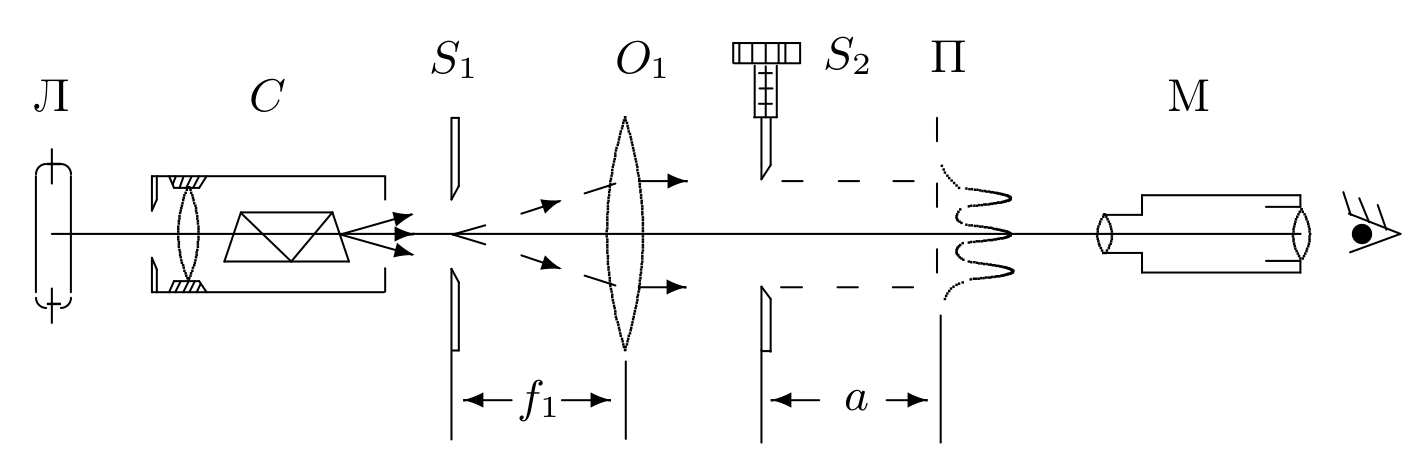
\includegraphics[width=1\linewidth]{scheme.png}}
		\caption{Схема установки для наблюдения дифракции Френеля}
		\label{img: scheme0}
	\end{figure}

	Щель $S_2$ освещается параллельным пучком монохроматического света с помощью коллиматора, 
	образованного объективом $O_1$ и щелью $S_1$, находящейся в его фокусе. На щель $S_1$ сфокусировано
	изображение спектральной линии, выделенной из спектра ртутной лампы $Л$ при помощи простого
	монохроматора $C$, в котором используется призма прямого зрения.

	Распределение интенсивности света в плоскости наблюдения $П$ проще всего рассчитывать с помощью зон
	Френеля (для щели их иногда называют зонами Шустера). При освещении щели $S_2$ параллельным пучком
	лучей (плоская волна) зоны Френеля представляют собой полоски, параллельные краям щели (рис. 2).
	Результирующая амплитуда в точке наблюдения определяется суперпозицией колебаний от тех зон Френеля,
	которые не перекрыты створками щели. Графическое определение результирующей амплитуды производится
	с помощью векторной диаграммы -- спирали Корню. Суммарная ширина $m$ зон Френеля $z m$ опре-
	деляется соотношением

	\begin{equation}
		z_m = \sqrt{a m \lambda}
	\end{equation} \label{eq::wide}
	\
	где $a$ -- расстояние от щели до плоскости наблюдения (рис. \ref{img: scheme0}), а $\lambda$ --
	длина волны

	Вид наблюдаемой дифракционной картины определяется числом Френеля $\Phi$: квадрат числа Френеля

	\begin{displaymath}
		\Phi^2 = \frac{D}{\sqrt{a \lambda}}
	\end{displaymath}
	\
	-- это отношение ширины щели D к размеру первой зоны Френеля, т.е. число зон Френеля, которые
	укладываются на ширине щели. Обратную величину называют волновым параметром

	\begin{displaymath}
		p = \frac{1}{\Phi^2} = \frac{D}{\sqrt{a \lambda}}
	\end{displaymath}


\section{Экспериментальная установка}
	


\section{Ход работы}

\end{document} % конец документа
